\section{Introduction--python functions }
  python has lots of pre-made functions , that you can use right now, simply by"calling"them. The concept of a function is one of the most important ones in mathematics.A common usage of functions in computer languages is to implement mathematical functions.Functions are a convenient way to divide your code into useful blocks, allowing us to order our code, make it more readable, reuse it and save some time. Also functions are a key way to define interfaces so programmers can share their code.

%this generates 1cm of vertical space

\section{  Defining a Function}

\begin{figure}[h!]
\centering
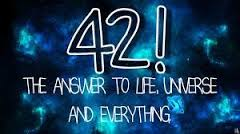
\includegraphics[scale=0.5]{universe.jpg}
\caption{The Universe}
\label{fig:univerise}
\end{figure}




  
 

 You can define functions to provide the required functionality. Here are simple rules to define a function in Python.

Function blocks begin with the keyword def followed by the function name and parentheses ( ( ) ).

Any input parameters or arguments should be placed within these parentheses. You can also define parameters inside these parentheses.

The first statement of a function can be an optional statement - the documentation string of the function or docstring.

The code block within every function starts with a colon (:) and is indented.

The statement return [expression] exits a function, optionally passing back an expression to the caller. A return statement with no arguments is the same as return None.













\section{Generator Functions }
Generators are a simple and powerful possibility to create or to generate iterators. On the surface they look like functions, but there is both a syntactical and a semantic difference. Instead of return statements you will find inside of the body of a generator only yield statements, i.e. one or more yield statements. 

The following is a simple example of a generator, which is capable of producing four city names:




\begin{verbatim}
def city_generator():
    yield("Konstanz")
    yield("Zurich")
    yield("Schaffhausen")
    yield("Stuttgart")
\end{verbatim}

 It's possible to create an iterator with this generator, which generates one after the other the four cities Konstanz, Zurich, Schaffhausen and Stuttgart. 

\begin{verbatim}
>>> from city_generator import city_generator
>>> x = city_generator()
>>> print x.next()
Konstanz
>>> print x.next()
Zurich
>>> print x.next()
Schaffhausen
>>> print x.next()
Stuttgart
>>> print x.next()
Traceback (most recent call last):
  File "<stdin>", line 1, in <module>
StopIteration
>>> 
\end{verbatim}
